\chapter{Tentang Docker}

\begin{chapquote}{Docker, \textit{docker.com}}
    ``Docker makes development efficient and predictable''
    \end{chapquote}

\section{Pengertian Docker}

\noindent Dikutip dari situs Docker Docs, Docker merupakan aplikasi open source untuk developing, shipping dan running aplikasi. 
Docker memungkinkan aplikasi untuk terpisah dari infrastrukturnya, sehingga proses deliveri aplikasi dapat dilakukan dengan cepat.
\begin{figure}
    \begin{center}
        
\includegraphics[width=\linewidth]{image/docker.PNG}
        \caption{Docker}
        \label{fig:my_figure1}
    \end{center}
\end{figure}

Docker menyediakan kemampuan untuk mengemas dan menjalankan aplikasi di lingkungan yang terisolasi yang disebut container.
Dengan konsep isolasi dan security docker pengguna dapat menjalankan banyak container secara bersamaan pada host tertentu. Container berisi 
semua yang diperlukan untuk menjalankan aplikasi, sehingga tidak perlu bergantung pada apa yang saat ini terinstall pada host. Selain itu
pengguna dapat berbagi container dengan mudah.


\section{Keuntungan Menggunakan Docker}
\noindent Penggunaan docker mempunyai beberapa keuntungan bagi penggunanya baik developer ataupun perusahaan. 
Berikut merupakan keuntungan menggunakan docker : 
\begin{enumerate}
    \item Cepat dan konsisten dalam deliveri aplikasi
    \item Kontainer docker dapat berjalan dimana saja, baik lokal, mesin fisik/virtual, cloud provider, dan lingkungan campuran lainnya
    \item Menjalankan lebih dari 1 kontainer dalam satu perangkat yang sama
    \item Ukuran kontainer yang relatif kecil
    \item Hemat biaya dalam perangkat sehingga dengan spesifikasi hardware yang kurang namun banyak komputasi yang dijalankan
\end{enumerate}


\section{Arsitektur Docker}
Dikutip dari situs Docker Docs, Docker menggunakan struktur client-server. Docker client dapat berkomunikasi dengan Docker daemon yang menjalankan tugas untuk membangun, 
menjalankan, dan mendistribusikan container docker. Docker client dan docker daemon dapat berjalan dalam sistem yang sama, ataupun 
secara remote/jarak jauh. docker client dan docker daemon berkomunikasi menggunakan REST API melalui socket UNIX atau interface jaringan. 
Docker client lainnya yaitu Docker Compose yang memungkinkan client untuk berkomunikasi dengan aplikasi yang didalamnya terdapat banyak 
container

\begin{figure}
    \begin{center}
        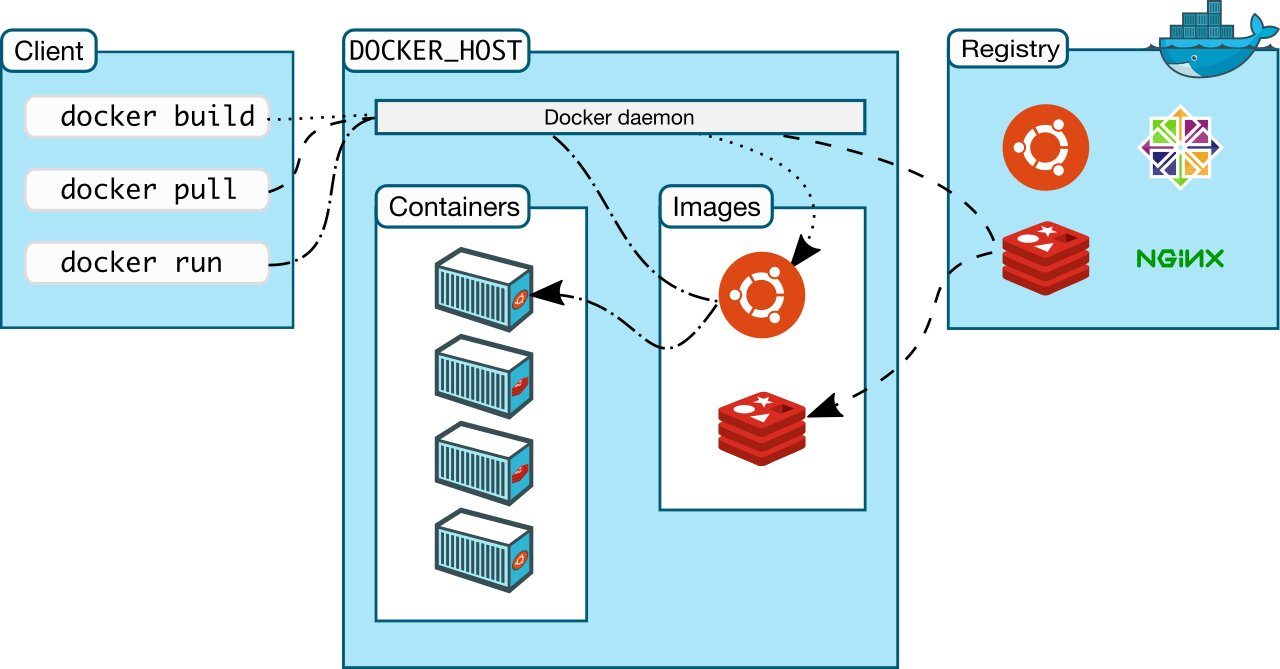
\includegraphics[width=\linewidth]{image/architecture.jpg}
        \caption{Arsitektur Docker}
        \label{fig:my_figure2}
    \end{center}
\end{figure}


\subsection{Docker Daemon}
Docker daemon/dockerd mendengarkan permintaan Docker API dan mengelola objek docker seperti images, container, networks dan volume. 
Docker daemon juga dapat berkomunikasi dengan daemon lain untuk mengelola layanan docker.

\subsection{Docker Client}
Docker client merupakan pengguna docker. Saat pengguna menjalankan perintah seperti run maka docker client akan mengirimkan perintah 
ini ke dockerd dan menjalankannya. Menggunakan docker API dan dapat berkomunikasi lebih dari satu daemon.

\subsection{Docker Desktop}
Docker desktop merupakan aplikasi versi GUI dari docker untuk pengguna yang ingin berinteraksi dengan docker lewat tampilan.

\subsection{Docker Registries}
Docker registries merupakan registri publik untuk menyimpan docker images yang dapat diakses oleh publik. Pengguna juga dapat membuat 
registri/repositori sendiri dan mengupload docker images pengguna ke registri docker. Saat menggunakan perintah docker pull atau docker run, 
docker image akan diambil dari registri yang dikonfigurasi, saat menggunakan perintah push docker images akan didorong/diupload ke registri 
yang dikonfigurasi. Docker registri yang dapat diakses secara publik yaitu docker Hub.

\subsection{Docker CE}
Docker CE atau Docker Community Edition adalah varian docker untuk developer dan small teams yang baru menggunakan docker dan melakukan 
experimen aplikasi berbasis container. Docker CE mempunyai 2 sumber update yaitu Stable dan Edge. Update stable yaitu update yang tersedia 
setiap tiga bulan sekali, dan Edge yaitu update setiap bulan.

\subsection{Docker EE}
Docker EE atau Docker Enterprise Edition adalah varian docker untuk enterprise development dan IT teams. Docker EE terintegrasi, 
bersertifikat, dan didukung untuk menyediakan perusahaan dengan platform container paling aman di industri.


\subsection{Docker Object}

\subsubsection{Images}

Docker images merupakan template read-only yang digunakan untuk membangun container docker. Docker images dapat berisi images yang 
lain dan memuat detail konfigurasi yang diperlukan untuk membuat aplikasi berjalan dengan baik. Images dapat dibuat oleh pengguna 
ataupun menggunakan images yang diambil dari docker registries. Jika images dibuat oleh pengguna sendiri, maka pengguna membuat 
Dockerfile yang berisi sintaks dan langkah yang diperlukan untuk menjalankan aplikasi dalam images. Docker images lebih ringan, 
kecil dan cepat jika dibandingkan dengan teknologi virtualisasi lainnya.

\subsubsection{Container}

Container merupakan wadah/tempat untuk menjalankan aplikasi secara isolasi/terpisah dari lingkungan infrastruktur. Container berisikan 
docker images yang dapat dijalankan. Pengguna dapat membuat, memulai, menghentikan, memindahkan atau menghapus container menggunakan 
Docker API atau CLI. Dengan container pengguna dapat menjalankan lebih dari satu container dalam satu host, kemudahan dalam distribusi 
dan pengujian aplikasi, dan terintegrasi baik secara lokal, cloud, dan hybrid sekalipun.